%%% VCU thesis/dissertation template file

%%%%%%%%%%%
\makeatletter
\let\my@xfloat\@xfloat
\makeatother
% Create a modified copy of \@xfloat using the kernel definition
%%%%%%%%%%%

\documentclass[copyright, reqno]{vcuthesis}
\makeatletter
\def\@xfloat#1[#2]{
        \my@xfloat#1[#2]%
        \def\baselinestretch{1}%
        \@normalsize \normalsize
}
\makeatother
%% http://www.latex-community.org/forum/viewtopic.php?f=45&t=4766&start=10#p33170
%%%%%%%%%%%%

% PACKAGES %

% CHNGCNTR resets counter
\usepackage{chngcntr}

%%%%%%%%%%%
% GRAPHICX for figures
\usepackage{graphicx}

% AMSMATH package for equations
\usepackage{amsmath}

% SUBFIGURE package for sub-figures
\usepackage{subfigure}

% BIBLATEX package for bibliography
\usepackage[sorting=none]{biblatex}

% APPENDIX package for information in Appendix sections
\usepackage[titletoc]{appendix}

% HYPERREF enables URLs to Figures/Sections/Chapters/Tables
\usepackage[linktocpage=true]{hyperref}

%%%%%%%%%%%

% BIBLIOGRAPHY %

%%%%%%%%%%%
\bibliography{references} % uses treferences.bib file
\renewcommand{\type}{Thesis}
\renewcommand{\thetable}{\arabic{table}}
\newcommand{\comments}[1]{}
%%%%%%%%%%%

% EQUATIONS %

%%%%%%%%%%%
% will be numbered with respect to chapter
\numberwithin{equation}{chapter}
%%%%%%%%%%%

% DOCUMENT  %

%%%%%%%%%%%
\begin{document}
\pagenumbering{roman}

% Edit the following accordingly %

%%%%%%%%%%%
\newcommand{\thesistitle}{Dissertation Title}
\newcommand{\authorsname}{Student Name}
\newcommand{\thesismonth}{December}
\newcommand{\graduatingyear}{2013}
\newcommand{\degree}{Doctor of Philosophy}
\newcommand{\pastdegreeone}{Student degree with university - Dates} % Example:  September 2000 to April 2004
% If more than one degree, uncomment and use below command. Also uncomment line 897 [ which is {\pastdegreetwo}] in vcuthesis.cls file
%\newcommand{\pastdegreetwo}{Student degree with university - Dates} % Example:  September 2006 to April 2006
\newcommand{\committeechair}{Dissertation director's name}
\newcommand{\major}{Director Department}
\newcommand{\chairposition}{Director Title}

\vspace*{10em}
\begin{center}
\thispagestyle{empty}
\copyright Candidate Name, December {\graduatingyear}\\
All Rights Reserved.
\end{center}
\vspace*{\fill}
\maketitlepage

% ACKNOWLEDGEMENTS  %

\acknow{
Rebum fabellas ea ius, mea electram ullamcorper no, et sed graece offendit nominati. Id vel nonumy commune sadipscing, eros philosophia pri ne, ea duo splendide hendrerit deterruisset. Eam delectus constituto ex, usu ad quot tollit adipisci. Quando mollis corrumpit ea mel, omnium singulis neglegentur id mea. Ut usu nostro audire forensibus. Ei eam errem minimum deserunt, oblique interesset eu vel, te erroribus ocurreret vix. 
}

\pagestyle{plain}
\tableofcontents
%\listofalgorithms
\listoftables
\listoffigures
%\clearpage

\setlength{\headheight}{12pt}

% ABSTRACT  %

\theabstract{ \label{sec:abstractlabel}
Rebum fabellas ea ius, mea electram ullamcorper no, et sed graece offendit nominati. Id vel nonumy commune sadipscing, eros philosophia pri ne, ea duo splendide hendrerit deterruisset. Eam delectus constituto ex, usu ad quot tollit adipisci. Quando mollis corrumpit ea mel, omnium singulis neglegentur id mea. Ut usu nostro audire forensibus. Ei eam errem minimum deserunt, oblique interesset eu vel, te erroribus ocurreret vix
}\\

\clearpage

\pagenumbering{arabic}
%%% put your main text here
\chapter{Introduction \label{chap:chapintro} }
Section \ref{sec:background} desribes the background of this dissertation.
\section{ Section in a chapter \label{sec:background} }
Rebum fabellas ea ius, mea electram ullamcorper no, et sed graece offendit nominati. Id vel nonumy commune sadipscing, eros philosophia pri ne, ea duo splendide hendrerit deterruisset. Eam delectus constituto ex, usu ad quot tollit adipisci. Quando mollis corrumpit ea mel, omnium singulis neglegentur id mea. Ut usu nostro audire forensibus. Ei eam errem minimum deserunt, oblique interesset eu vel, te erroribus ocurreret vix \cite{Narendra_1990}. Figure \ref{fig:fig1} describes quick brown fox jumps over the dog.

% Figure %
\begin{figure}
\centering
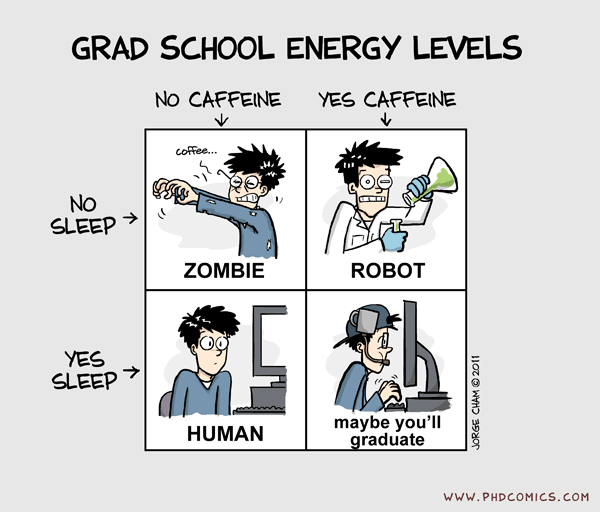
\includegraphics[scale=0.6]{figures/phd.png}
\caption{Grad School Energy Levels}
\label{fig:fig1}
\end{figure}

% Table %
\begin{table}
	\caption{\label{table:t1} Table Title}
	\vspace{0.15in}
	\centering
	\resizebox{3cm}{!}{
	% To change number of columns from 3 to 4, change {l l l} below to {l l l l }. For lines between columns, use {l | l | l}
	\begin{tabular} {l l l} \hline \hline
		{\bf C1} & {\bf C2} & {\bf C3} \\ \hline
		a & b & cc \\
		01 & 3 & 0.7 \\
		10 & string & string \\
		31 & 63 & 127 \\ \hline \hline
	\end{tabular}
	}
\end{table}

\subsection{Sub-section One}
Rebum fabellas ea ius, mea electram ullamcorper no, et sed graece offendit nominati. Id vel nonumy commune sadipscing, eros philosophia pri ne, ea duo splendide hendrerit deterruisset. 
\subsection{Sub-section Two}
Eam delectus constituto ex, usu ad quot tollit adipisci. Quando mollis corrumpit ea mel, omnium singulis neglegentur id mea. Ut usu nostro audire forensibus.
\subsection{Sub-section Three}
Eam delectus constituto ex, usu ad quot tollit adipisci. Quando mollis corrumpit ea mel, omnium singulis neglegentur id mea. Ut usu nostro audire forensibus.

\chapter{Literature Review \label{chap:litreview}}
This document follows the VCU dissertation guidelines listed at:\\ \href{http://www.graduate.vcu.edu/pdfs/Thesis\%20and\%20Dissertation\%20Manual\%20Fall\%202012.pdf}{VCU Dissertation Manual [PDF]}
\chapter{Methodology \label{chap:methods}}
\section{Using Equations}
Equation \ref{eqn:tfcombEQ3} represents ..

\begin{equation}
F_{2}(G_{i}, T_{j}) = \dfrac{B^{1}_{i,j}}{\sum\limits_{k=1}^{t}B^{1}_{i,k}} + \dfrac{B^{2}_{i,j}}{\sum\limits_{k=1}^{t}B^{2}_{i,k}}
\label{eqn:tfcombEQ3}
\end{equation}

\section{Using Mathematical Expressions}
Use mathematical expressions between dollar symbols (as shown) for unique representation within a paragraph.
$-0.5*\log (P_{1}P_{2})$ \\

Eam delectus constituto ex, usu ad quot tollit adipisci. Quando mollis corrumpit ea mel, omnium singulis neglegentur id mea. Ut usu nostro audire forensibus. Following methods are used:
% ENUMERATE is used for listing %
\begin{enumerate}
\item Method 1
\item Method 2
\item Method 3
\end{enumerate}

\section{Using Sub-figures}
Figure \ref{fig:secondthree} shows sub-figures.
PDFs can also be imported to create a figure.

\begin{figure}
\centering
	\subfigure[Algorithm Complexity]{
		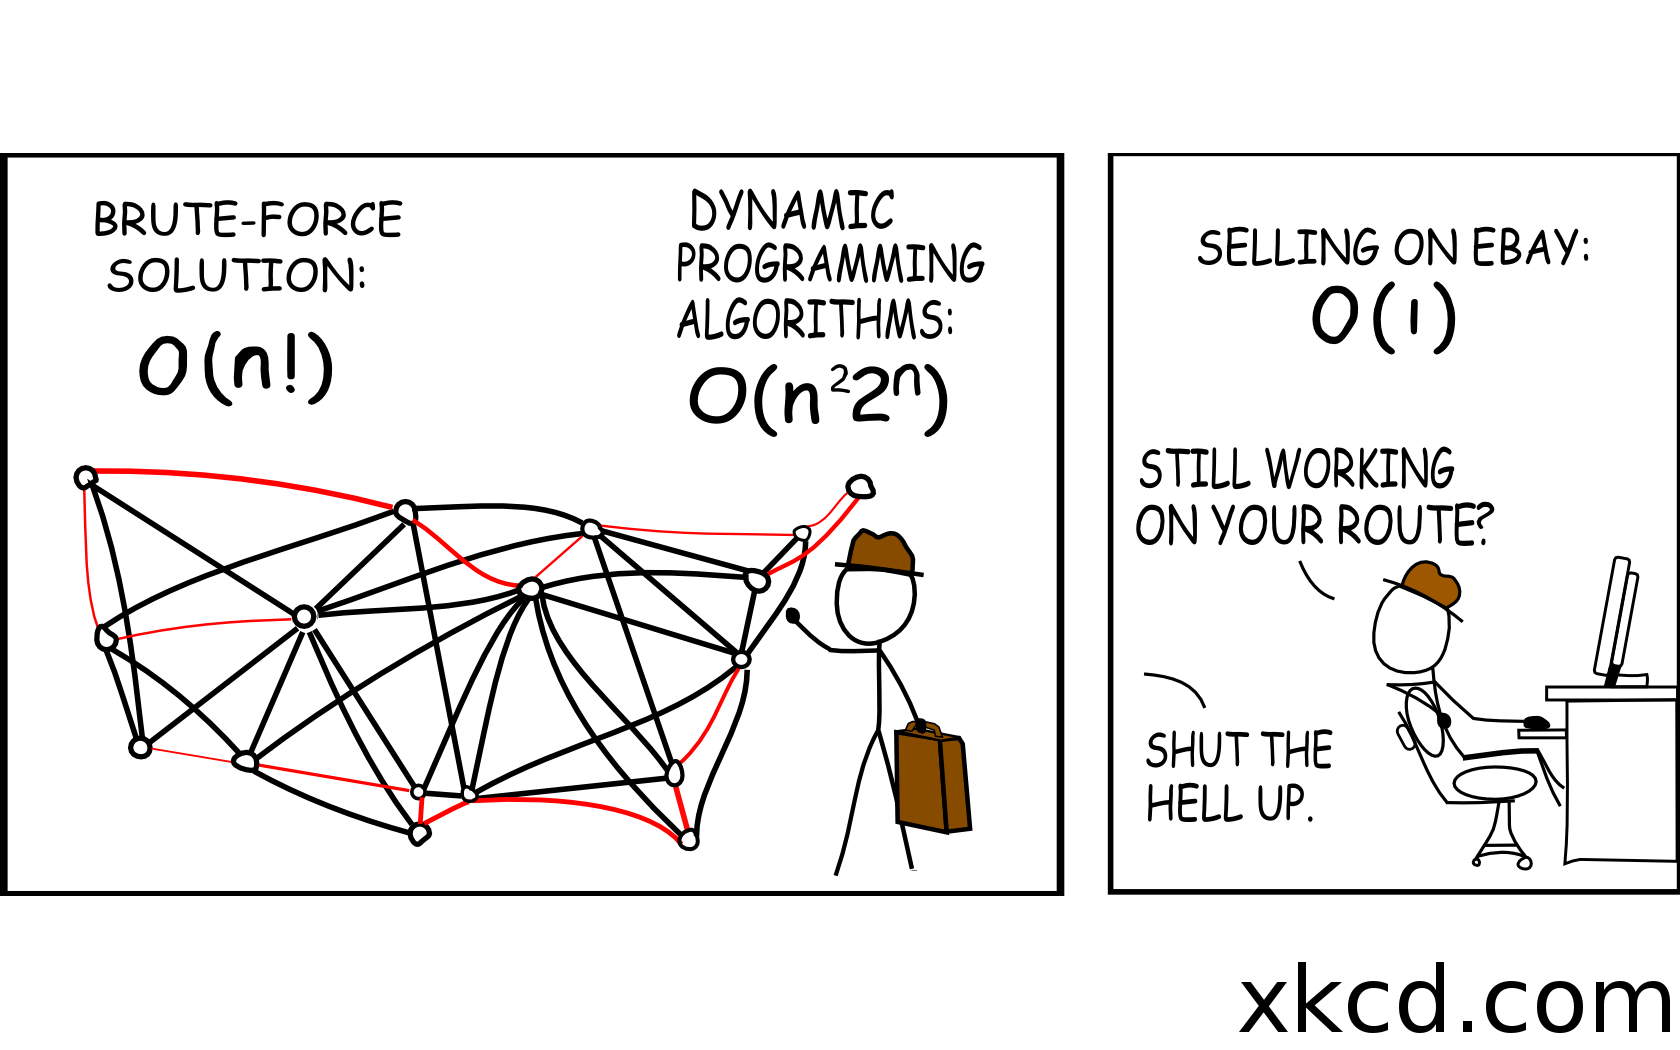
\includegraphics[scale=0.5]{figures/xkcd_vd.png}
		\label{fig:secondFig}
}
\end{figure}
\begin{figure}
\centering
	\subfigure[Python import antigravity]{
		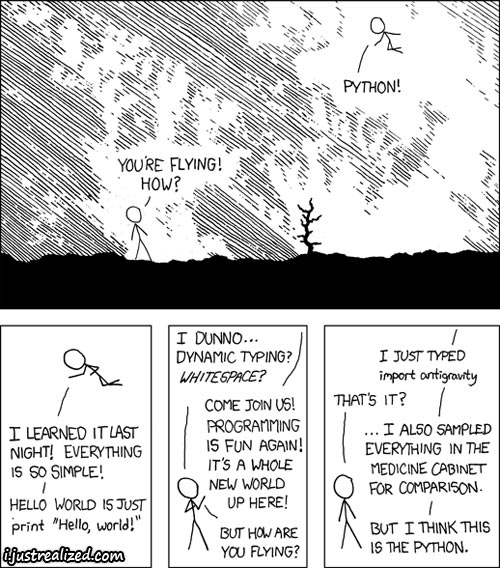
\includegraphics[scale=0.5]{figures/xkcd-python.jpg}
		\label{fig:secondsecondFig}
}
\end{figure}
\begin{figure}
\centering
	\subfigure[Perl]{
		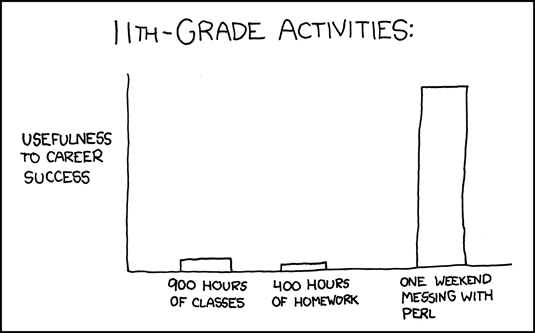
\includegraphics[scale=0.5]{figures/11th_grade.png}
		\label{fig:secondthirdFig}
}
	\caption{Comics from \emph{XKCD} }
\label{fig:secondthree}
\end{figure}

\chapter{Results \label{chap:resultschap}}

% APPENDIX  %
\begin{appendices}
\chapter{Abbreviations}
\begin{tabular}{ll}
VCU &Virginia Commonwealth University \\
RVA & Richmond Virginia \\
\end{tabular}
\end{appendices}

\begin{appendices}
\chapter{Other}
Rebum fabellas ea ius, mea electram ullamcorper no, et sed graece offendit nominati. Id vel nonumy commune sadipscing, eros philosophia pri ne, ea duo splendide hendrerit deterruisset. Eam delectus constituto ex, usu ad quot tollit adipisci. Quando mollis corrumpit ea mel, omnium singulis neglegentur id mea. Ut usu nostro audire forensibus.
\end{appendices}

\printbibliography[title={References}, heading=bibintoc]

\chapter*{Vita}
\thispagestyle{plain}
\addcontentsline{toc}{chapter}{Vita}
Rebum fabellas ea ius, mea electram ullamcorper no, et sed graece offendit nominati. Id vel nonumy commune sadipscing, eros philosophia pri ne, ea duo splendide hendrerit deterruisset. Eam delectus constituto ex, usu ad quot tollit adipisci. Quando mollis corrumpit ea mel, omnium singulis neglegentur id mea. Ut usu nostro audire forensibus.

\end{document}
